\documentclass{article}
    \usepackage{pgfplots}
    \pgfplotsset{compat=1.8}
    \usepgfplotslibrary{statistics}
    \begin{document}
    
    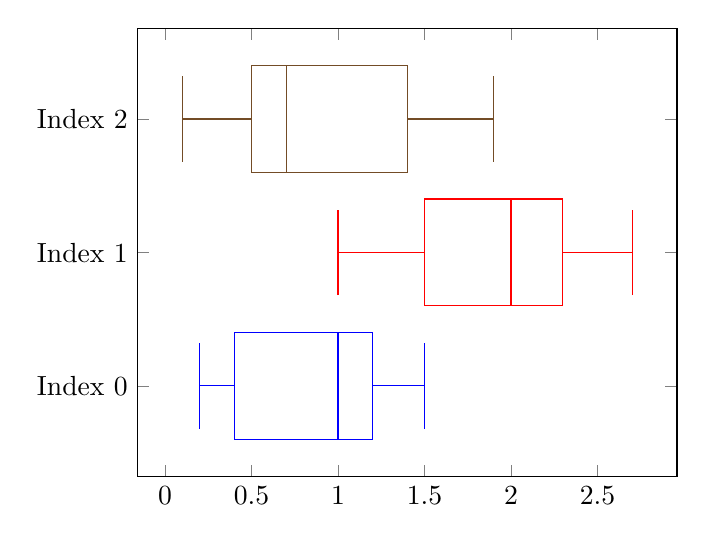
\begin{tikzpicture}
      \begin{axis}
        [
        ytick={1,2,3},
        yticklabels={Index 0, Index 1, Index 2},
        ]
        \addplot+[
        boxplot prepared={
          median=1,
          upper quartile=1.2,
          lower quartile=0.4,
          upper whisker=1.5,
          lower whisker=0.2
        },
        ] coordinates {};
        \addplot+[
        boxplot prepared={
          median=2,
          upper quartile=2.3,
          lower quartile=1.5,
          upper whisker=2.7,
          lower whisker=1
        },
        ] coordinates {};
        \addplot+[
        boxplot prepared={
          median=0.7,
          upper quartile=1.4,
          lower quartile=0.5,
          upper whisker=1.9,
          lower whisker=0.1
        },
        ] coordinates {};
      \end{axis}
    \end{tikzpicture}
    
    \end{document}